\documentclass[10pt]{beamer}

\usepackage[francais]{babel}

\usetheme{metropolis}           % Use metropolis theme

\usepackage{listings}

\usepackage{booktabs}
\usepackage[scale=2]{ccicons}

\usepackage{pgfplots}
\usepgfplotslibrary{dateplot}

\title{Interfaces Utilisateur Graphiques}
\subtitle{Projet C}
\date{\today}
\author{Pierre Bouvier, Maxime Gourgoulhon, Julie Saouli}
\institute{Ensimag}
% \titlegraphic{\hfill\includegraphics[height=1.5cm]{logo/logo}}

\begin{document}

\maketitle

\begin{frame}
  \frametitle{Table des matières}
  \setbeamertemplate{section in toc}[sections numbered]
  \tableofcontents[hideallsubsections]
\end{frame}

\section{Organisation du projet}

\begin{frame}[fragile]
	\frametitle{Organisation du projet.}

    Nous avons utilisé \emph{Github} pour travailler en groupe et gérer aussi le code que les tâches via le système de \textbf{tickets}.

    Globalement nous avons travaillé ensemble à l'ENSIMAG.

    \begin{center}
    \begin{figure}
	   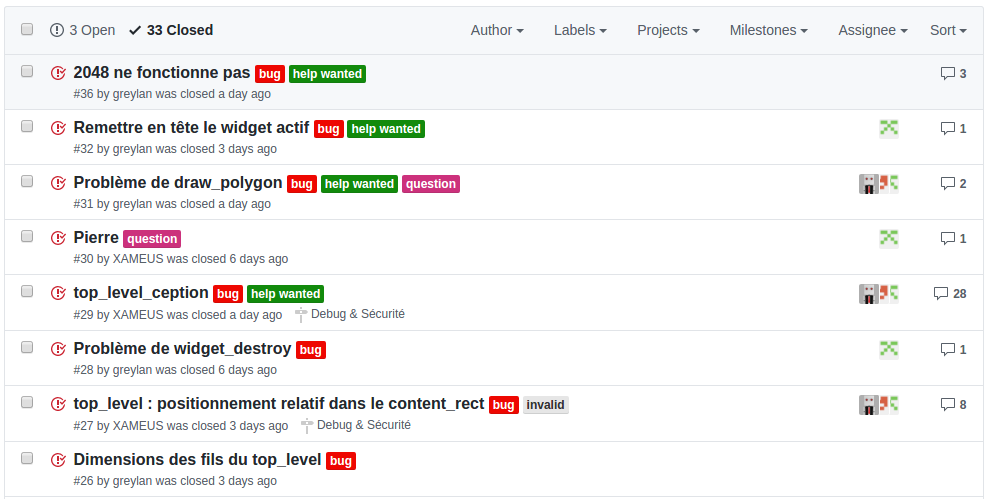
\includegraphics[width=10cm]{capture0.png}
    	\caption{Github : l'outil pour travailler en groupe :)}
    \end{figure}
    \end{center}

    % \hfill \emph{wikipédia}
\end{frame}

\section{Ce qui a été fait}

\begin{frame}{État du programme vis à vis du cahier des charges.}

    \begin{enumerate}
        \item \textbf{Primitives de dessin} : ei\_map\_rgba, ei\_draw\_polyline, ei\_draw\_polygon, ei\_draw\_text, ei\_fill, ei\_copy\_surface, \emph{ei\_draw\_text\_lines}, \emph{ei\_draw\_diamond}
        \item \textbf{Placeur}: ei\_place, ei\_placer\_run, ei\_placer\_forget
        \item \textbf{Widgets}: ei\_frame\_t, ei\_button\_t, ei\_toplevel\_t, \emph{ei\_radiobutton\_t}
        \item \textbf{Évènements}: ei\_event\_set\_active\_widget, ei\_event\_get\_active\_widget, ...
    \end{enumerate}

\end{frame}
\lstset{
basicstyle=\footnotesize, frame=tb,
xleftmargin=.2\textwidth, xrightmargin=.2\textwidth
}
\begin{frame}{Choix "intéressants" : callback list}

\end{frame}

\begin{frame}{Choix "intéressants" : INVALIDATE\_RECT}

\end{frame}

\begin{frame}{Choix "intéressants" : struct ei\_frame\_t}
    \begin{center}
        \lstinputlisting[language=C]{source0.c}
    \end{center}
\end{frame}

\section{Ce qui a été fait (en plus) :D}

\begin{frame}{ei\_draw\_text\_lines}
    \textbf{Un} seul texte, pour \textbf{plusieurs} lignes !
\end{frame}


\begin{frame}{ei\_radiobutton\_t}
    Ils sont beaux, ils sont radios !
\end{frame}

\section{Tests en directs !}

\plain{Questions ?}

\end{document}
